\section{Introduction}

The delivery of cargo by means of automotive transport is an important stage among distribution processes. The final stage of delivery to the client’s door known as the “Last Mile” is a particularly important part of this process. Studies show that precisely this stage is one of the most expensive and most complicated ones in organization. That’s why many modern developments are focused on the optimization, improvement and simplification of this process.

So, for example, the vehicle route optimization system was developed to reduce delivery costs through better route planning for all vehicles, which in turn allows vehicles to handle more points of delivery at a time and therefore reduces the overall number of required vehicles \cite{art1}. Such a result is very important not only for economical reasons, but also ecological ones, because reducing the number of vehicles being used also means a reduction in the amount of harmful substances emitted into the atmosphere.

Unfortunately, while implementing vehicle route optimization systems, many problems emerge related to the fact there are always various deviations from a plan that during deliveries, no matter how optimal it is. The correction of the plan through communication with a dispatch operator are required every time for corresponding deviations.

Experience shows that expediter drivers and couriers start to perform deliveries without following the plan if the process of communication with the dispatch operator and plan correction is insufficiently simple and effective. For example, the need to call the dispatch operator every time or to use a program for recording extraordinary situations on a smart phone with touch-sensitive control detains the driver and distracts him from the main task of driving a vehicle.

In modern vehicle-mounted systems, voice control elements appear increasingly frequently \cite{art2,Kravchenko_2009,Heisterkamp_2001}. Besides that, the use of a voice interface helps to free the driver’s hands and simplifies the process of gathering additional statistical information, which in turn facilitates and improves the planning of the next routes \cite{conf9}. Unfortunately, the best modern voice recognition systems cannot be installed on a mobile device and work only in online mode. Yet for the task of distribution, it can be hard to ensure access to the Internet at any time, because the delivery destination may be located in places/regions that do not even have mobile GPRS Internet or where the data transfer speed is too low to work with sound. So the request for the further improvement of voice interaction automation is important for improving the effectiveness of the distribution system.

\section{Literature data analysis and problem statement}

The Japanese researcher Ishiguro Hiroshi from Osaka University and his colleagues studied different aspects of communication and information and communication technology, such as the usage of communication with human-like robots as a therapeutic practice for senior citizens \cite{Nishio_2015}, autistic persons \cite{Kumazaki_2016} or just people withdrawn into themselves, or as a pedagogical practice for children and babies \cite{Park_2015} etc. In particular, he conducted studies on indirect voice communication between two persons via computers \cite{Ishiguro_2016}.

In this study, the couple communicated on common issues selecting variants of their remarks from the option tree written in advance, some kind of script. Neither of the partners had to say anything out load: a person was provided with a set of reply options to choose from, and all they needed to do was to press on the remark which the given person would have liked to say and this remark was played from speakers. Depending on the remark used, the program selected possible reply options from an option tree and presented them to the communicating partner to choose from. After having heard the remark of the first person, the communicating partner in turn selected his/her own remark from the options given. This study was aimed at overcoming shyness while communicating with persons of the opposite sex (which is particularly important for Japan). However, this approach of using a tree of communication scripts written in advance can be used in other spheres as well. 

In his speech at the Global Psychological Congress 2016, Professor Ishiguro demonstrated the usage of this scenario approach for robots at exhibitions and in museums.  To avoid the necessity for voice recognition in a noisy environment, a human-like robot and a display showing question options are put next to an exhibit item. By pressing different remarks, a visitor can speak with the robot according to the script tree written in advance and pose questions to the robot about the exhibit item, and the robot answers with voice. 

Unfortunately, the reverse task arises for distribution management – the driver has to enter certain information into the system while not being distracted by pressing buttons on a display. The direct usage of such technology is thus not possible. However, using the approach of describing all possible communication scripts depending on the context will allow the amount of information that has to be recognized to be reduced and thus improve quality \cite{art2}. 

Most modern speech recognition systems are based on statistical methods and use powerful machinery of probability theory and the mathematical statistics that enables the essential improvement of recognition quality. Hidden Markov models and artificial neural networks are the main methods of speech recognition \cite{Makovkin_2006, Gefke_2012}. However, models based on neural networks are more widespread in modern systems, because they have a greater response speed and noise tolerance \cite{Hinton_2012}.

The recognition of a voice command and its transformation into the text one is a traditional approach to solving the problem. A fairly large number of such systems exists, and they fulfil their task quite qualitatively. However, in terms of the qualitative recognition of the arbitrary signal into the text, the system needs to be quite large and include big context-sensitive vocabularies. This is precisely the reason why the best modern speech recognition systems such as Google Voice Search cannot be installed on mobile devices and work only in online mode. Unfortunately, for the task of distribution, it can be hard to ensure access to the Internet at any time, because the delivery destination may be located in places/regions that do not even have mobile GPRS Internet or where the data transfer speed is too low to work with sound. 

A new approach to voice control exists at the moment that is based on the theory of unforced interaction \cite{Teslia_2010} – a reflex system of voice control \cite{Egorchenkov_2016}. The idea lying at the foundation of this approach is that instead of transferring voice information into the text representation, the information component has to be analysed directly, identifying which of the known responses needs to be performed. «Traditional systems of speech recognition are based on the principle of: “oral speech” → “speech representation by the set of linguistic constructions” → “speech understanding”. On the basis of the theory of unforced interaction, another model of natural language recognition can be suggested: “oral speech” → “estimation of unforced (informational) interaction on responses” → “response (understanding or behaviour)”» \cite{Teslia_2014}. 

Such a recognition model is called a reflex model, because it is built by analogy with the structure of the conditional reflex in which affecters, the central component and effectors are distinguished. This model can be well connected with the idea of the script tree usage, because scripts also consist of responses and not a linguistic peculiarity of speech but a response (or command) that can be taken into account by the automated system of the route calculation becomes a unit of modelling. Thus, the essence of this approach lies in transferring to another unit of speech recognition. The experience of speech analysis through the segregation of the other units - functional expressions are also accumulated in the psychology of discursive thinking and reflexive psychology \cite{Naydonov_2008}. 

Since vocabularies, complicated intelligent models of text and grammar analysis are not needed in such a system, they possess a number of advantages in comparison with traditional systems: multi-diction, variability of natural language, possibility of offline command processing directly on a device, working in noise conditions (acoustically uncontrolled environment), simplicity of algorithms and lower complexity and price of realization \cite{Teslia_2013}. 

The problem is that existing methods of voice interaction automation can’t accomplish tasks of distribution due to the contradiction between conditions of such activity and the required powers of devices for the recognition of a voice signal into a text one being used in most of the known models. The idea is that the development of a voice interaction model without a unit for transferring the sound of voice into text can essentially improve the voice interaction automation in systems for distribution control. 

The hypothesis is suggested that combining the two most promising trends found in the result of analyses provides the possibility to offer a new fundamental decision and to build a reflex model of voice interaction in tasks of distribution control. 

\section{The purpose and tasks of the research}

The purpose of the Study is to improve the effectiveness and convenience of drivers’ work in distribution systems through the development and usage of intelligent reflex systems of voice interaction without a unit for transferring the sound of voice into text that will provides the possibility to automate certain processes of distribution management, thus improving the level of service and reducing costs.

The task is to adopt the use of intelligent reflex systems of voice control for tasks of distribution and to compare the effectiveness of different options for the realization of such systems by creating a context model of voice interaction in systems for the dispatch control of vehicle traffic. 

\section{Materials and study methods}

\subsection{The script tree as a method for the presentation of content and contexts of voice interaction}

The context model of voice interaction is based on logical scripts of interaction on the topic of distribution control which have to take into account the criteria of main reasons for the deviation of the real situation from the planned route, e.g. late arrivals or refusals to perform the service at the point of delivery etc \cite{art3}. This makes it possible to get information for making a decision on the return of cargo to the warehouse, on cancellation or postponement of the service at one point of delivery in order to use a possibility to be on time at another, more important point of delivery, on a route change to avoid a traffic jam or on the creation of a new route with a standby vehicle etc. 

As for the presentation of the script tree, the best choice is the directed graph in which nodes define the system status (contexts) and dialogue phrases which the system will voice and edges define the content of driver’s remarks (stimuli) which can be perceived by the system in every certain node. A response to the stimulus can result in a transfer between statuses, and the directed edge is thus drawn from the node in which the stimulus can be perceived to the node which shows in what status the system will transfer in response to the stimulus. So the set of all edges coming from the node define the list of stimuli between which the recognition has to be performed for the status corresponding to this node. 

Each node of the graph defines the system context that limits possible remarks which the system can perceive in this status. This approach allows the the quality of recognition to be significantly improved by means of decreasing the number of possible responses. Moreover, it helps to shorten commands, because the necessity for their global uniqueness is eliminated. The same context can be in several nodes simultaneously if these nodes have the same set of edges coming out such nodes. 

\subsection{The method of intelligent reflex systems for the creation of a voice control reflex system} 

The method of intelligent reflex systems was used to create the system for the formalization of voice interaction. The method is created on the basis of the theory of unforced interaction – the computer model of the world in which the real movement is described as stochastic movements with the speed of light at the subatomic level. The formulas derived from this movement model were used for the description of the interaction of arbitrary objects and for modelling statistic patterns in the text \cite{Teslia_2010}. 

As for the reason for the creation of intelligent reflex systems, it is suggested that the dependence of the combined conditional probability of the response on the unconditional probability of the response and partial conditional probabilities of the response in this system is subordinated to the laws of conservation of momentum in the computer model and that they can be calculated according to the corresponding formulas. 

The reflex method for the calculation of the adequate response to the set of different weakly structured incoming influences is the algorithmic basis of such systems. 

The implementation scheme of this method includes the following stages:

1. The calculation of determination for an intelligent system regarding all incoming influences and possible responses.

An analogy of determination of responses and influences in computer model of the world is an impulse of material objects. Two groups of objects are discussed in this model – those that make an impact through the “collision” and transfer of their own information (an impulse) to objects on which the impact is made (according to possible responses): 

\[
d(A_i)=\pm0.5\sqrt{\frac{p(A_i)}{1-p(A_i)}+\frac{1-p(A_i)}{p(A_i)}-2};
\]

\[
i(A_i)=\sqrt{d^2(A_i)+1};
\]

\[
d(A_i/B_j)=\pm0.5\sqrt{\frac{p(A_i/B_j)}{1-p(A_i/B_j)}+\frac{1-p(A_i/B_j)}{p(A_i/B_j)}-2};
\]

\[
i(A_i/B_j)=\sqrt{d^2(A_i/B_j)+1},
\]

\noindent
where: $p(A_i)$ — unconditional probability of selecting response $A_i$; $d(A_i)$ — determination regarding response $A_i$; $i(A_i)$ — information awareness regarding response $A_i$; $p(A_i/B_j)$ — conditional probability of selecting response $A_i$ (upon the existence of impact $B_j$); $d(A_i/B_j)$ — determination regarding response $A_i$ in the case of impact $B_j$; $i(A_i/B_j)$ — information awareness regarding response $A_i$ in the case of impact $B_j$.

2. From the informational and probabilistic interpretation of the formula of the relativistic velocity addition, an additional determination is derived that influencing objects have regarding responses (velocity of movements of influencing objects regarding objects being influenced): 

\[
\Delta d(A_i/B_j)=d(A_i/B_j)\cdot i(A_i)-d(A_i)\cdot i(A_i/B_j)
\]

\noindent
where $\Delta d(A_i/B_j)$ — additional determination regarding response $A_i$ provided by influence $B_j$. 

3. From the informational and probabilistic interpretation of the law of conservation of momentum, the total impact on the response of the intelligent system is calculated. An analogue of “hit” of many moving objects (corresponding actions) on objects corresponding to responses

\[
d_\Sigma(A_i) = \sum_j \Delta d(A_i/B_j); \\
\]

\[
i_\Sigma(A_i) = \sqrt{\Delta d^2(A_i/B_j)+1},
\]

\noindent
where $d_\Sigma(A_i)$ — the total additional determination regarding response $A_i$ under the impact of all events $B_j$ ; $i_\Sigma(A_i)$ — total supplementary awareness regarding response $A_i$ under the impact of all events $B_j$. 

4. The new determination of responses is calculated (an analogue of new velocity of movement after the impulse received during the collision with influencing objects)

\begin{equation}
\label{eq:ifron2}
d(A_i/B)=d_\Sigma(A_i)\cdot i(A_i)+d(A_i)\cdot i_\Sigma(A_i),
\end{equation}


\[
i(A_i/B) = \sqrt{d^2(A_i/B)+1},
\]

\noindent
where $d(A_i/B)$ — new determination regarding response $A_i$ with account of the impact of all events $B_j \in B$; $i(A_i/B)$ — new information awareness regarding response $A_i$ with account of the impact of all events $B_j \in B$.

5. It is possible to calculate the combined conditional probability of response $A_i$, if necessary (upon the existence of all impacts $B_j \in B$)

\[
p(A_i/B)=0.5+\frac{d(A_i/B)}{2i(A_i/B)};
\]

\noindent
where $p(A_i/B)$ — combined conditional probability of response $A_i$ (upon the existence of all impacts $B_j \in B$).

To formalize voice information, a system was used that consists of two main modules: the automatic phonetic stenographer and the core of the reflex system of voice control (RSVC), the current implementation of which defines the conditions of their usage in the model of voice interaction of the driver during the dispatch control of vehicle traffic (image \ref{img:rsgu_struct}).

\begin{figure}[htb]
	\centering
	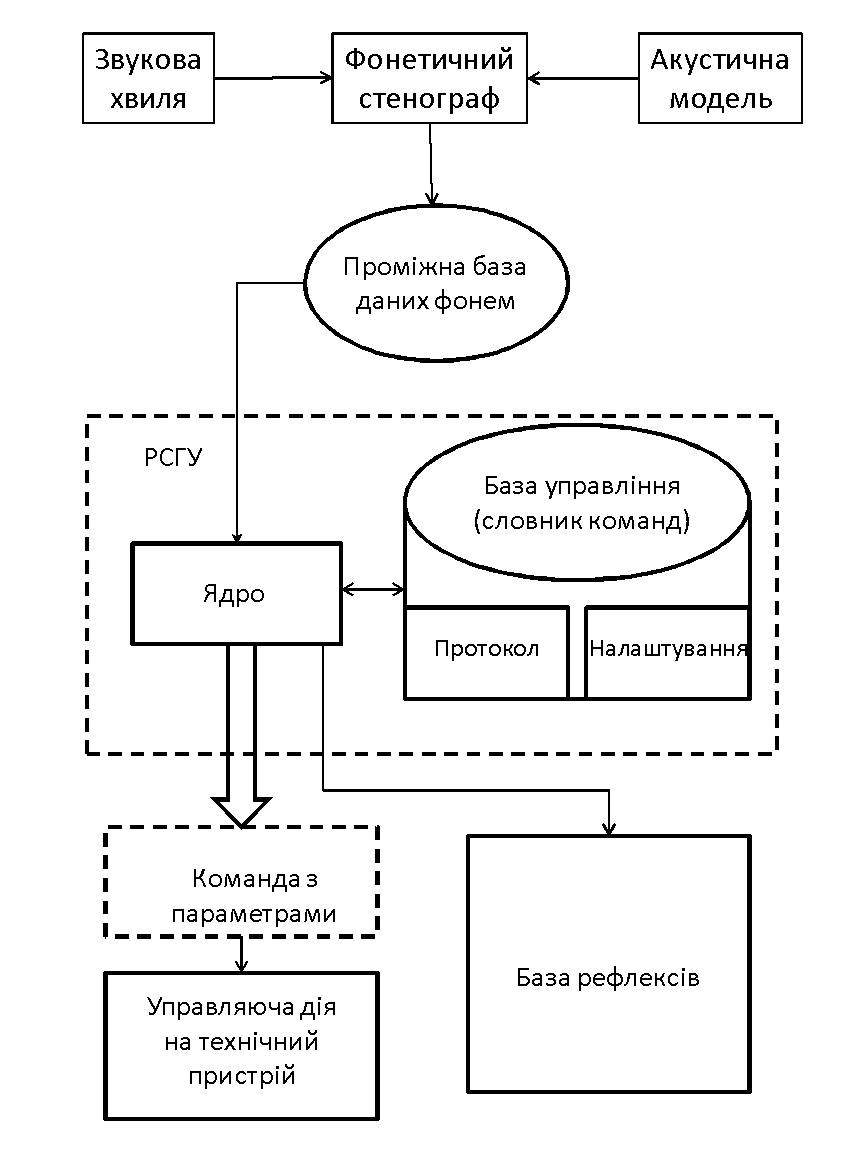
\includegraphics [width=.5\linewidth] {rsgu_struct}
	\caption{The structure of the system of voice information formalization in the model of voice interaction of the driver during the dispatch control of vehicle traffic}
	\label{img:rsgu_struct}
\end{figure}

The usage of the phonetic stenographer algorithm allows the creation of a sequence of contexts for a speech signal without the use of any vocabulary. For this reason, certain generative grammar is built that can synthesize all possible model signals of uninterrupted speech for any sequence of phonemes. Within this built model, the algorithm of phoneme-by-phoneme recognition is constructed for an unknown signal with the usage of contexts and possible responses to them. 

In the reviewed system of voice information formalization (image \ref{img:rsgu_struct}), the voice command serves as incoming information which can be represented by a sound wave; and the process of managing the impact on the controlled object will serve as outgoing information, and the realization of the recognized command will thus take place according to the parameters previously set by the voice. 

The system of voice information formalization itself will generate needed screen and voice informational messages for the driver in the course of work, which will in turn provide the possibility to monitor the process of recognizing commands, responses to them, and moreover, it will allow the system behaviour to be changed on a real time basis, if necessary. 

\section{Results of voice command classification in systems of distribution control} 

\subsection{Description of the developed context model of voice interaction in systems for the dispatch control of vehicle traffic} 

Statistical data, feedback and comments on the process of different cargo deliveries by vehicles in leading logistics companies were gathered to create a context model of voice interaction in systems for the dispatch control of vehicle traffic. Having organized and processed gathered original comments on the delivery status which are used in different companies, a script tree was developed for subjects of distribution “depot – road – point of delivery” \cite{art3}. 

The complete script tree of all distribution stages “depot – road – point of delivery” in the context model of the driver’s voice interaction in the system of dispatch control of vehicle traffic is shown in Image \ref{img:13_complete_scenario_graph}.

\begin{figure}
	\centering
	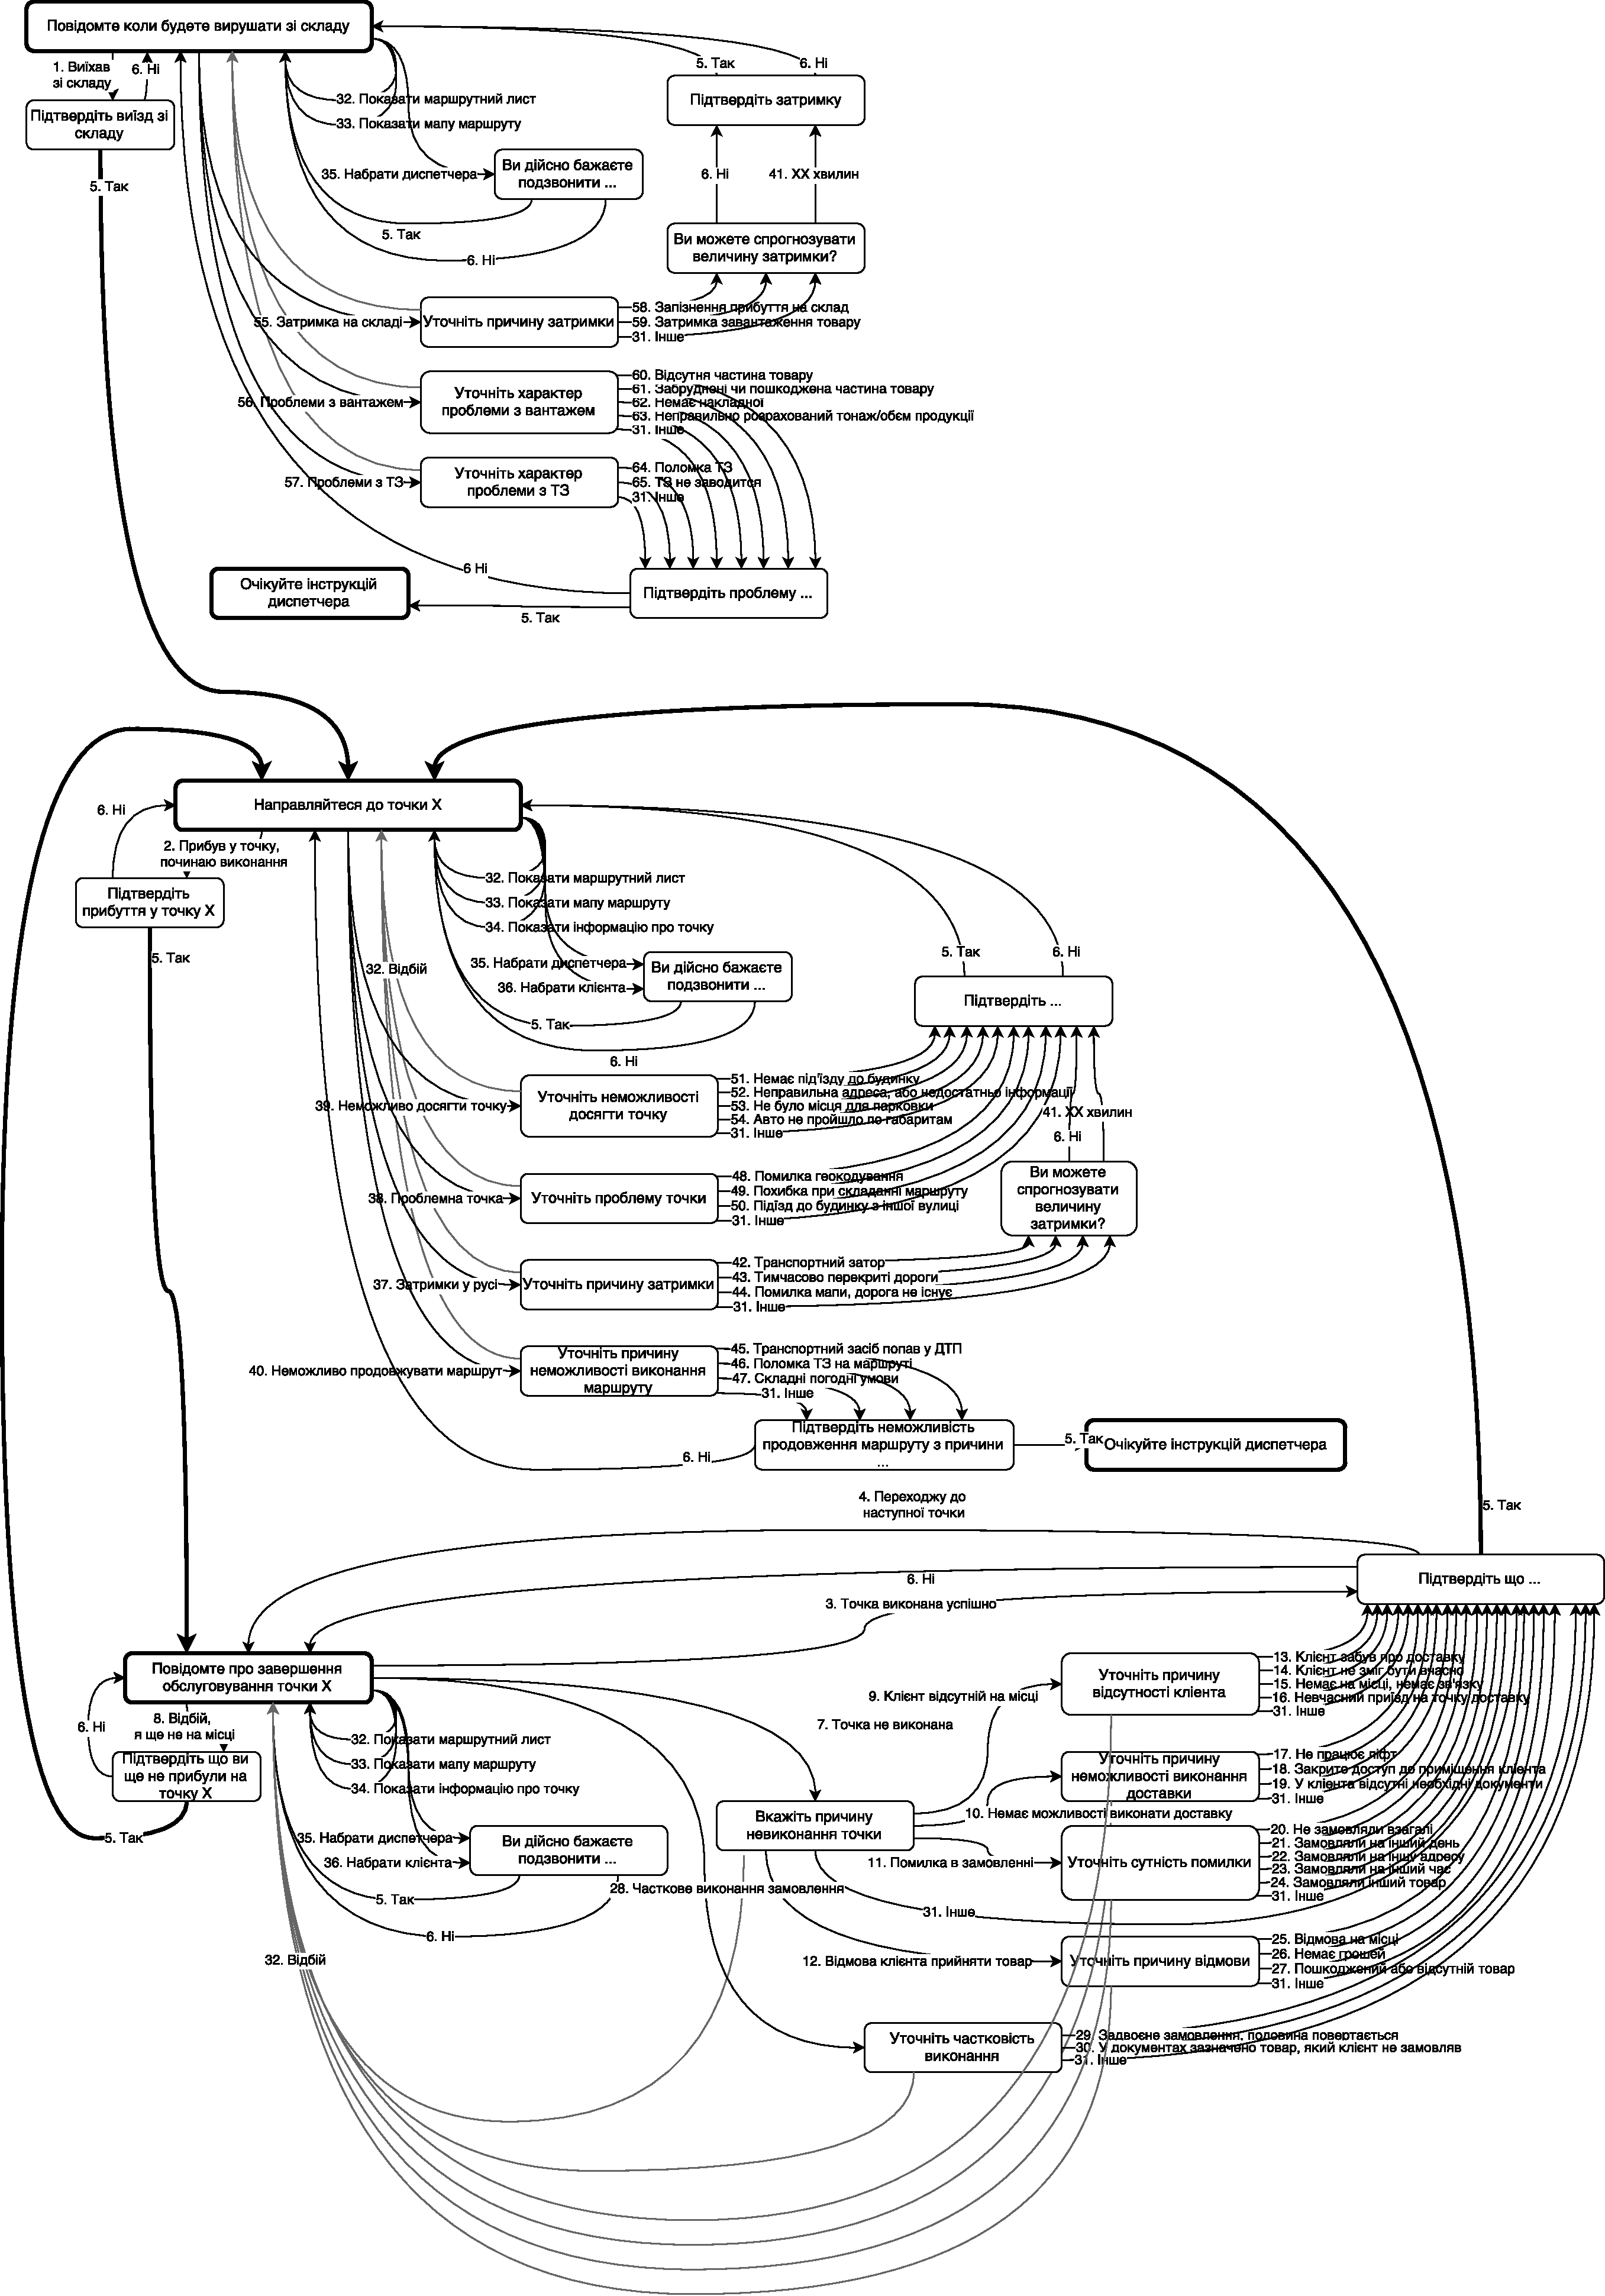
\includegraphics [width=1\linewidth] {13_complete_scenario_graph}
	\caption{Complete script tree of voice interaction}
	\label{img:13_complete_scenario_graph}
\end{figure}

In the complete script tree of all distribution stages (Image \ref{img:13_complete_scenario_graph}), most possible reasons for being late or failing to fulfil the stages “depot”, “road”, and “point of delivery” are taken into account, and for cases where there is no possibility to fulfil the stage, the indication (instructions) of the dispatch operator exists on the further actions of the driver.

From the mentioned script tree, unique contexts based on possible remarks which have to be recognized in any of the contexts were highlighted and enumerated. These data are specified in Table \ref{tbl:context_reactions}.

\begin{table} [!htb]%
	\caption{The list of contexts and possible responses in them}%
	\label{tbl:context_reactions}
	\def\tabularxcolumn#1{m{#1}}
	\centering
	\begin{tabularx}{0.7\textwidth}{@{}>{\centering}m{3.0cm} | >{\raggedright\arraybackslash}X@{}}
		\toprule
		№ Контексту & Можливі реакції	\\
		\midrule
		1 & 5, 6 \\
		2 & 6, 41 \\
		3 & 1, 32, 33, 35, 55, 56, 57 \\
		4 & 8, 31, 58, 59 \\
		5 & 8, 31, 60, 61, 62, 63 \\
		6 & 8, 31, 64, 65 \\
		7 & 2, 32, 33, 34, 35, 36, 37, 38, 39, 40 \\
		8 & 8, 31, 51, 52, 53, 54 \\
		9 & 8, 31, 48, 49, 50 \\
		10 & 8, 31, 42, 43, 44  \\
		11 & 8, 31, 45, 46, 47 \\
		12 & 3, 7, 8, 28, 32, 33, 34, 35, 36 \\
		13 & 4, 5, 6 \\
		14 & 8, 9, 10, 11, 12, 31 \\
		15 & 8, 13, 14, 15, 16, 31 \\
		16 & 8, 17, 18, 19, 31 \\
		17 & 8, 20, 21, 22, 23, 24, 31 \\
		18 & 8, 25, 26, 27, 31 \\
		19 & 8, 29, 30, 31 \\
		\bottomrule
	\end{tabularx}
\end{table}

As is shown on the structure chart (Image \ref{img:rsgu_struct}), the system of voice information formalization consists of two main modules: phonetic stenographer for the transfer of the voice signal in the text phoneme-by-phoneme representation and the core of the reflex system of voice control (RSVC), which classifies the text phoneme-by-phoneme representation according to a given set of possible commands. 

In the capacity of the module of the phonetic stenographer for the Ukrainian language, previous development is used \cite{Pylypenko_2008} and made in the form of a binary application, a set of libraries and configuration files for the Windows platform. 

In the capacity of the RSVC core, the intelligent reflex system based on the theory of unforced interaction can be used. For this reason, the phonemes of each remark were divided into sequential sets of phonemes of different lengths known as N-grams in methods of the text processing. To use the formulas mentioned above, it was necessary to define the unconditional probability of selection for every response and the conditional probability of selection of every response upon the existence of the impact from any N-gram. These values were calculated statistically on the basis of an analysis of the set of text data. Then the combined conditional probability of the response upon the existence of impacts from all N-grams in the remark was calculated on the basis of the formulas mentioned above through information awareness and determination. 

The development of the RSVC core was performed in the JavaScript language in the node.js environment using the SQLite database. The opensource code of the developed system is in public access \cite{code1}. 

\subsection{The usage of the method of convolutional neural networks for the classification of the phoneme-by-phoneme representation of voice commands} 

The model based convolutional neural networks (CNN) was used to check the work of intelligent reflex systems. The model based CNN is an alternative implementation of the RSVC core from the chart in Image \ref{img:rsgu_struct}. 

The CNN for work with phonemes mostly plays a role similar to the CNN in the task of the text classification \cite{Kim_2014} but operates on the “text”, not word-by-word but phoneme-by-phoneme what looks like the work with the text character-by-character \cite{Zhang_2016}. 

The system built in the Python language with the use of TensorFlow framework based on the implementation of the CNN for work with the text \cite{Britz_2015}. The opensource code of the developed system is in public access \cite{code2}. 

The structure of the neural network can be represented as follows. 

Phonemes are represented in the form of one-hot vectors. Phrases are normalized over the maximum length, with the use of the vector with all zeros as filler.

Contrary to the work word-by-word, the embedding layer is absent because the power of a phonemic set is much lower than the power of a set of words and such a layer is not necessary. On the other hand, some phonemes are like others and other phonemes are not, so the use of embedding can be appropriate for the transfer of this likeness, but not only for lowering the dimensionality. Training the embedding layer requires a large amount of input data, so it won’t be discussed in this work. 

A combined convolution layer is used consisting of several parallel one-dimensional layers with different sizes of the filter. 

A pooling layer with the selection of one maximum value (1-max-pooling) is used for the aggregation of each convolution layer. 

Outputs of the pooling layers of a different convolution filter sizes are combined into one vector of values. 

The fully connected layer with ReLu activation function is used. Traditionally, the cross-entropy is used for tasks of classification as the loss function. The Adam-algorithm of the back propagation of error with the stochastic gradient descent is used for training \cite{art4}. 

\begin{table} [!hb]%
	\caption{Percentage of recognition of IRS and CNN}%
	\label{tbl:data_total}
	\def\tabularxcolumn#1{m{#1}}
	\begin{tabularx}{\textwidth}{@{}>{\centering}X | >{\centering}X >{\centering}X | >{\centering}X >{\centering}X | >{\centering\arraybackslash}X@{}}
		\toprule
		№ Контексту & Точність розпізнавання ЗНМ & Кількість розпізнаних стимулів ЗНМ & Точність розпізнавання ІРС & Кількість розпізнаних стимулів ІРС & Загальна кількість стимулів в контексті	\\
		\midrule
		1 & 92.0 & 92 & 85 & 85 & 100 \\
		3 & 99.4 & 348 & 86.6 & 303 & 350 \\
		4 & 99.0 & 198 & 87 & 174 & 200 \\
		5 & 98.0 & 294 & 83 & 249 & 300 \\
		6 & 97.5 & 195 & 83.5 & 167 & 200 \\
		7 & 95.6 & 478 & 77.4 & 387 & 500 \\
		8 & 98.7 & 296 & 85.7 & 257 & 300 \\
		9 & 97.2 & 243 & 88.8 & 221 & 250 \\
		10 & 96.4 & 241 & 86.4 & 216 & 250 \\
		11 & 96.4 & 241 & 82.4 & 206 & 250 \\
		12 & 95.1 & 428 & 75.1 & 338 & 450 \\
		13 & 94.0 & 141 & 84.1 & 122 & 150 \\
		14 & 95.0 & 285 & 73 & 219 & 300 \\
		15 & 92.0 & 276 & 78 & 234 & 300 \\
		16 & 96.8 & 242 & 84 & 210 & 250 \\
		17 & 95.1 & 333 & 64.6 & 226 & 350 \\
		18 & 93.6 & 234 & 74 & 185 & 250 \\
		19 & 98.0 & 196 & 82.5 & 165 & 200 \\
		По всій вибірці & 90.2 & 2885 & 63.7 & 2038 & 3200 \\	
		\bottomrule
	\end{tabularx}
\end{table}

The modelling results according to both mentioned methods are given in Table \ref{tbl:data_total}. Dimensions of N-grams during the modelling by intelligent reflex systems were selected in the range of 2--4. Sizes of convolution filters during the modelling by convolutional neural networks were also selected in the range of 2--4.

\section{The discussion of results of modelling according to different methods and prospects for further studies}

Voice data of 23 different speakers (11 women and 12 men) were gathered for the experimental validation of the effectiveness of the developed methods. These persons dictated 64 responses present in the script tree (Image \ref{img:13_complete_scenario_graph}) using different variants of command formulations. A total of 3200 voice samples of commands were gathered. The data were processed by a phonetic stenographer and are in public access together with the outgoing code of models \cite{code1,code2}. 

The data were divided into training and test sets by means of a cross-validation method with the use of 5 groups. In other words, the data were randomly divided into 5 groups and modelling was conducted 5 times using each of the 5 groups as the test set and another 4 as the training one. Such an approach allows for the better evaluation of the precision of the method, because each of the data samples participates in the evaluation.

As we can see from Table \ref{tbl:data_total}, the convolutional neural networks showed a better result for classification of the set of phonemes into commands. 

We can also see that the lowest percentage of recognition during the use of both methods is demonstrated in the situation where contexts are not utilized and the simultaneous modelling of all teams takes place. From this, we can draw the conclusion that the use of the tree of scripts and contexts is viable. 

It was also noted during the different studies that training during the use of the IRS method is quicker than during the CNN method but that the actual recognition on the trained system is performed more quickly when convolutional neural networks are used. 

By taking a thorough looking at the core of the IRS calculations, it can be seen that it greatly resembles the fully connected layer of the neural network. The conditional probability of selection of response $A_i$ upon the existence of impact $B_j$ ($p(A_i/B_j)$) corresponds with the weights of the neural network layer ($W = |w_ij|$), and the unconditional probability of selection of response $A_i$ ($p(A_i)$) corresponds with the biases ($B = |b_i|$). In contrast to the classic perceptron in which the function of activation applies to the result of the matrix composition ($Y=f(WX + B)$), the activation function in the RSVC is a lot more complicated. Furthermore, it works with the weights and biases directly as, for example, the radial basis activation function. 

In the method of intelligent reflex systems, specifications $p(A_i/B_j)$ and $p(A_i)$ are calculated by frequency. When this method is actually in use, there is no training stage similar to that during the training of neural networks. Such an approach is more similar to the least squares method, where the parameters can be calculated directly and don’t need the optimization. 
However, if you limit the range of possible values of parameters by the interval $[0, 1]$ which corresponds with possible values of probability, then you can try to receive the optimal values of these parameters by means of the training using back propagation. 

The preliminary processing of phonemes (the combination of N-grams of phonemes of a different length) corresponds with the convolution and pooling layers of the convolution neural network, but the fixed set is used instead of the training of the best filters. It includes all possible combinations of phonemes (N-grams) according to the size of the filter’s window. Such fixed set of filters is, at the same time, a lot bigger than the one necessary for the effective recognition and is still not full enough, because it does not include nonlinear combinations and omissions when certain phonemes in the filter’s window are more important. So the training of optimal parameters of the filter in the neural network can provide better result. 

The function of activation of the RSVC is complicated enough, and its calculation is a lot longer than ReLU or other functions of activation of fully connected layers. Since the iterative learning is absent in the classic approach of the RSVC, it is not a critical issue. However, only the comparison of the introformation function of activation with classic features of neural networks’ nonlinearity in equal conditions can provide an independent evaluation of its effectiveness. 

\section{Conclusions}

The analysis of the distribution practice demonstrated that, during the implementation of vehicle route optimization systems, the necessity to simplify communication with the dispatch operator to correct routes after emerging for recording extraordinary situations remained unsatisfied. The main weakness of programs for recording extraordinary situations on devices with touch-sensitive control lies in the fact that the driver is detained and distracted from the main task of driving the vehicle, which in most cases leads drivers to avoid the route correction and carry out the delivery without adhering to the plan. The main weakness of modern systems of voice recognition lies in the fact that they need access to the Internet at all times and that the quality of the tools that can be installed on the phone is insufficient for speech recognition. 

In the work, the model of formalization of voice information in systems for the dispatch control of vehicle traffic is suggested, with the use of the script tree for modelling the voice interaction between the driver and the vehicle dispatching support systems and the intelligent reflex system of voice control for the classification of the voice commands described in the script tree.

A context model of the voice interaction of the driver in vehicle traffic dispatch control systems in the form of a communication script tree that allows the highlighting of contexts of voice commands recognition, thus allowing a variety of commands to be reduced and the quality of recognition to be improved, is developed. Due to the analysis of gathered statistical data, feedback and comments on different cargo delivery processes with vehicles in leading logistics companies, a complete tree of scripts of all the stages of distribution (“depot – road – point of delivery”) was suggested with the indication of contexts and with the inclusion of possible responses in them. 

The method of intelligent reflex systems of voice control was further developed. It was suggested that other methods for the classification of phoneme sets in commands be used as the core component of the system.  An alternative classifier of commands with use of the method of convolutional neural networks was developed. 

The modelling of the reflex system of voice control in systems for the dispatch control of vehicle traffic was carried out on the basis of voice data gathered from 23 different speakers (11 women and 12 men) who dictated 64 responses present in the script tree using different variants of command formulations. The modelling was performed using two alternative command classifiers in the capacity of the core component of the RSVC: with use of the method of intelligent reflex systems and convolutional neural networks. 

The analysis of the modelling results demonstrated that the use of the script tree and division of the complete set of commands in contexts is viable because the values of accuracy without the use of contexts are the lowest for both methods of classification. The comparison of modelling results for different methods of classification demonstrated that both methods can be used in a real-case scenario and the training of the model when using the method of intelligent reflex systems runs a lot more quickly than it does for convolutional neural networks, but an actual recognition on the trained system runs more quickly with the utilization of convolutional neural networks. The accuracy of modelling is also higher when using convolutional neural networks. 

Common features of methods of convolutional neural networks and of intelligent reflex systems were defined, and prospects for further studies on their comparison in more independent conditions were outlined. 

Due to the conducted study, an intelligent reflex system of voice control was developed and set and ready for implementation, which will allow the effectiveness and convenience of the work of drivers in distribution systems to be improved and will provide the possibility to automate distribution processes in the “last mile” stage, improve the level of service and reduce costs. 

